% !TEX root = ../Thesis.tex
% !TEX output_directory
\documentclass[11pt,a4paper,english,greek,twoside]{../Thesis}
\usepackage{diagbox}

\begin{document}
\chapter{Πειραματικά Αποτελέσματα} \label{chap:Results}

\section{Αποτελέσματα Offline ανάλυσης}

\subsection{Μεθοδολογία Εξαγωγής Αποτελεσμάτων}

\par Όπως αναφέραμε και στην υποενότητα \ref{subsec:experimental_setup}, 2 άτομα συμμετείχαν στην καταγραφή των δεδομένων, και καθένα από αυτά πήρε μέρος σε 4 διαφορετικές συνεδρίες. Ο λόγος που χρειάστηκαν τόσες, ήταν για να δοκιμάσουμε διαφορετικές παραμέτρους όσον αφορά την ΕΟΔ. Συγκεκριμένα, πειραματιστήκαμε με δύο διαφορετικές τιμές duty cycle (50\%, 75\%) καθώς και δύο διαφορετικές ομάδες συχνοτήτωv. Η πρώτη ομάδα είναι $F_{low} = [6Hz,7Hz,8Hz,9Hz]$, και η δεύτερη $F_{mid} = [12Hz,13Hz,14Hz,15Hz]$.

\par Τα είδη των αλγορίθμων με τους οποίους θα πειραματιστούμε είναι δύο. Αυτοί που δεν χρειάζονται δεδομένα εκπαίδευσης (PSD, PSD-GM, CCA) και αυτοί που χρειάζονται (PSD-PCA-MLR-kNN). Για την αξιολόγηση του αλγορίθμου της δεύτερης κατηγορίας, χρησιμοποιήσαμε leave-one-out cross validation (loocv), δηλαδή για κάθε δείγμα κρατούσαμε αυτό ως δείγμα δοκιμής (test data) και το ταξινομούσαμε χρησιμοποιώντας το εκάστοτε μοντέλο που εκπαιδεύαμε με βάση τα εναπομείναντα δείγματα (train data).

\par Μια άλλη παράμετρος για την οποία θα παρουσιάσουμε αποτελέσματα είναι το μέγεθος του κάθε epoch στο οποίο εφαρμόζεται ο εκάστοτε αλγόριθμος. Επιπλέον θα σχολιάσουμε την ικανότητα του συστήματος μας να ανιχνεύει την NC κατάσταση, παρουσιάζοντας τα confidence score διαφόρων περιπτώσεων, και καταλήγοντας σε ένα βέλτιστο κατώφλι $Thr_{NC}$

\par Αρχικά θα παρουσιάσουμε τα αποτελέσματα για κάθε μία από τις τέσσερις συνεδρίες προκειμένου να καταλήξουμε στην βέλτιστη επιλογή συχνοτήτων και duty cycle. Στην συνέχεια θα παρουσιάσουμε την συνολική πιστότητα του συστήματος αλλά και τους αντίστοιχους ITR, για διάφορα χρονικά παράθυρα, μόνο για τις εντολές IC (Intentional Control) και χωρίς να συμπεριλαμβάνουμε την NC, καθώς αυτός είναι και ο τρόπος που παρουσιάζονται γενικά τα αποτελέσματα σε παρόμοιες εργασίες. Έπειτα, θα ασχοληθούμε με την NC κατάσταση, όπου θα προσπαθήσουμε να βρούμε το κατάλληλο κατώφλι $Thr_{NC}$, και θα παρουσιάσουμε τα αποτελέσματα των μεθόδων, με τον ίδιο τρόπο που έγινε για τις IC. Τέλος, θα μελετήσουμε τα κύματα άλφα, το πως θα γίνεται η ανίχνευση τους, και τα ποσοστά ταξινόμησης τους.

\subsection{Επιλογή συχνοτήτων και duty cycle (d.c), για χρονικό παράθυρο t=5sec}
\label{subsec:total_results}

\par Έπειτα από σχολαστική ανασκόπηση της βιβλιογραφίας, παρατηρήσαμε πως σχεδόν πάντα το ποσοστό επιτυχίας μιας μεθόδους, βελτιώνεται όσο αυξάνεται το παράθυρο υπολογισμού (διάρκεια epoch). Γι' αυτό το λόγο, θα παρουσιάσουμε τα συνολικά αποτελέσματα και για τις 4 συνεδρίες κάθε ατόμου, για $t=5sec$, έτσι ώστε να επιλέξουμε αρχικά τις βέλτιστες συχνότητες και τιμές duty cycle, για τον καθένα, όντας σχεδόν σίγουροι πως η επιλογή μας δεν θα άλλαζε αν ελέγχαμε μικρότερα χρονικά παράθυρα. 

\begin{table}[H]
    \centering
    \begin{tabular}{ |p{4cm}||p{1cm}|p{1cm}|p{1cm}|p{1cm}|p{1cm}|p{1cm}|p{1cm}|p{1cm}|}
        \hline
        \multicolumn{1}{|c||}{}& \multicolumn{8}{c|}{Χρήστης S1}\\
        \hline
        & \multicolumn{4}{c|}{$F_{low}$} & \multicolumn{4}{c|}{$F_{mid}$} \\
        \hline
        & \multicolumn{2}{c|}{$50\%$} & \multicolumn{2}{c|}{$75\%$} &
        \multicolumn{2}{c|}{$50\%$} & \multicolumn{2}{c|}{$75\%$} \\
        \hline
        & \multicolumn{1}{c|}{$A_c$} & \multicolumn{1}{c|}{$ITR$} &
         \multicolumn{1}{c|}{$A_c$} & \multicolumn{1}{c|}{$ITR$} &
          \multicolumn{1}{c|}{$A_c$} & \multicolumn{1}{c|}{$ITR$} &
           \multicolumn{1}{c|}{$A_c$} & \multicolumn{1}{c|}{$ITR$} \\
        \hline
        PSD             & 0.7625&   9.99&  0.8125& 12.079& 0.7125&  8.14& 0.7625&   9.99 \\
        PSD-GM          & 0.8375&  13.22&    0.85& 13.82&  0.825& 12.64& 0.7875&  11.00 \\
        CCA             &  0.875&  15.09&    0.90& 16.47&   0.85& 13.82& 0.7625&   9.99 \\
        PSD-PCA-MLR-kNN & 0.8375&  13.22&    0.9125& 17.19&     0.8& 11.53&    0.8&  11.53 \\
        \hline
        mean            &  0.825&  12.88&   0.87& 15.49&   0.80& 11.53& 0.77&   10.63 \\
        \hline
        \multicolumn{5}{c}{}\\
        \hline
        \multicolumn{1}{|c||}{}& \multicolumn{8}{c|}{Χρήστης S2}\\
        \hline
        & \multicolumn{4}{c|}{$F_{low}$} & \multicolumn{4}{c|}{$F_{mid}$} \\
        \hline
        & \multicolumn{2}{c|}{$50\%$} & \multicolumn{2}{c|}{$75\%$} &
        \multicolumn{2}{c|}{$50\%$} & \multicolumn{2}{c|}{$75\%$} \\
        \hline
        & \multicolumn{1}{c|}{$A_c$} & \multicolumn{1}{c|}{$ITR$} &
         \multicolumn{1}{c|}{$A_c$} & \multicolumn{1}{c|}{$ITR$} &
          \multicolumn{1}{c|}{$A_c$} & \multicolumn{1}{c|}{$ITR$} &
           \multicolumn{1}{c|}{$A_c$} & \multicolumn{1}{c|}{$ITR$} \\
        \hline
        PSD             & 0.6625&    6.51& 0.8375&  13.22& 0.7875&  11.00&  0.475&  2.03 \\
        PSD-GM          & 0.7125& 8.14&    0.8125& 12.07& 0.7625&  9.99&   0.5125&  2.73 \\
        CCA             & 0.8125& 12.07&   0.8875& 15.77& 0.8375& 13.22&   0.65&  6.13 \\
        PSD-PCA-MLR-kNN & 0.8125& 12.07&    0.85& 13.82&  0.7875& 11.00&  0.5875& 4.42 \\
        \hline
        mean            &  0.75&  9.70&   0.846& 13.72&   0.793& 11.30& 0.556& 3.83 \\
        \hline
    \end{tabular}
    \caption{Συγκεντρωτικά αποτελέσματα πιστότητας $A_c$ και ρυθμού $ITR (bits/min)$ κάθε χρήστη, για κάθε συνδυασμό συχνοτήτων ($F_{low}, F_{mid}$), duty cycle ($50\%, 75\%$), και μεθόδων που δοκιμάστηκαν, για χρονικό παράθυρο t=5sec}
    \label{tab:full_results}
\end{table}

\par Στον πίνακα \ref{tab:full_results}, παρουσιάζουμε τα αποτελέσματα για το πρόβλημα της ταξινόμησης των SSVEP στις τέσσερις κλάσεις, χωρίς να συμπεριλαμβάνουμε τις καταστάσεις NC και "κλειστά μάτια" (alpha κύματα). Για τις δύο διαφορετικές παραμέτρους ΕΟΔ που δοκιμάσαμε (duty cycle, συχνότητες) έχουμε να πούμε τα εξής. Είναι γεγονός, πως μεταξύ καθεμίας από τις τέσσερις συνεδρίες παρεμβάλλονταν αρκετές ώρες οι και μέρες, δηλαδή η κατάσταση του κάθε χρήστη διέφερε αρκετά. Συνεπώς, για να είμαστε απόλυτα σίγουροι πως αυτές οι αλλαγές που παρατηρούμε στις επιδόσεις, ευθύνονται στις διαφορετικές επιλογές duty cycle και συχνοτήτων, θα έπρεπε οι συνεδρίες να γίνουν τουλάχιστον την ίδια μέρα και διαδοχικά. Ωστόσο, παρατηρούμε μια συνέπεια και στους δύο χρήστες, όσον αφορά το γεγονός πως η χρήση χαμηλότερου d.c ευνοεί τις υψηλότερες συχνότητες, και αντίστροφα. Η παρατήρηση αυτή συμβαδίζει με τα αποτελέσματα που παρουσιάστηκαν στην δημοσίευση \cite{Huang2012-va} όπου φάνηκε πως το πλάτος των SSVEP σημάτων που αντιστοιχούσαν σε ΕΟΔ με συχνότητα 13Hz, ήταν μέγιστο για duty cycle 30\%, ενώ για συχνότητα 7Hz, το μέγιστο πλάτος παράχθηκε όταν χρησιμοποιήθηκε duty cycle 75\%. 

\par Τέλος, πρέπει να αναφέρουμε και τις παραμέτρους των μεθόδων που χρησιμοποιήθηκαν για τα παραπάνω αποτελέσματα. Για την PSD-GM, χρησιμοποιήσαμε τα πρώτα $k=20$ peaks του φάσματος για το κανάλι O1, και σε κάθε κάθε $Gm_i$ συνάρτηση, θέσαμε $N_h=3$, $a_{ih}=1/N_{h}$ και $\sigma_{ih}=0.1*h$ για $h=1,2,3$. Για την CCA, όμοια θέσαμε $N_h=3$, και χρησιμοποιήσαμε και τα τέσσερα κανάλια O1, O2, P7, P8. Στην συνδυαστική μέθοδο PSD-PCA-MLR-kNN, αρχικά χρησιμοποιήσαμε τα PSD σήματα των O1,O2. Για την PCA, ορίσαμε να κρατάει τις συνιστώσες που είναι υπεύθυνες για το 80\% του συνολικού variance, καθώς για μεγαλύτερες τιμές, γινόταν overfitting με αποτέλεσμα να μειώνεται η επίδοση, και για τον kNN χρησιμοποιήσαμε $k=5$ γείτονες.

\par Τελικώς, επιλέχθηκαν να μελετηθούν περαιτέρω, τα δεδομένα των συνεδριών που αντιστοιχούσαν στις συχνότητες $F_{low}$ με duty cycle 75\%, καθώς αυτά παρουσίασαν τα υψηλότερα ποσοστά πιστότητας, και για τους δύο χρήστες

\subsection{Αποτελέσματα για IC,  t=1-5sec}

\begin{figure}[H]
    \centering     %%% not \center
    \textbf{Χρήστης S1 (IC)}\par\medskip
    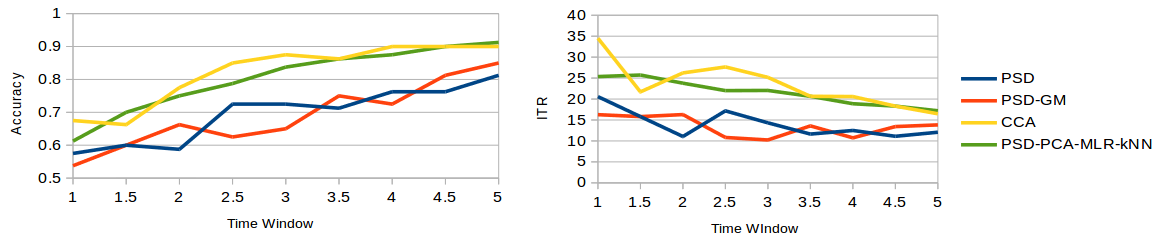
\includegraphics[scale=0.4]{{{ImagesSSVEP/S1_IC}.png}}
    \caption{Οι καμπύλες πιστότητας και ITR, του χρήστη S1, για διαφορετικές τιμές χρονικού παραθύρου}
    \label{fig:S1_graphs}
\end{figure}

\begin{figure}[H]
    \centering     %%% not \center
    \textbf{Χρήστης S2 (IC)}\par\medskip
    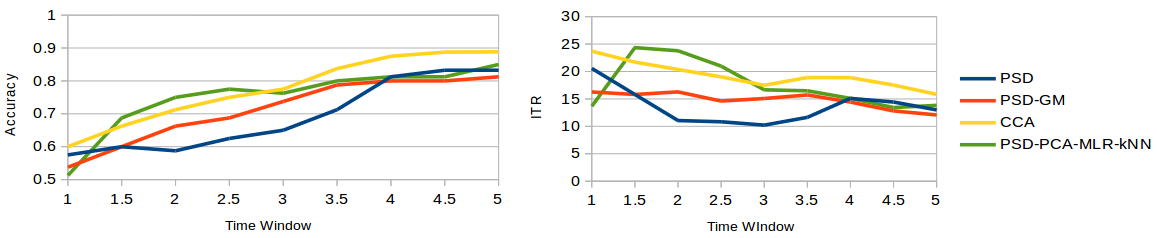
\includegraphics[scale=0.4]{{{ImagesSSVEP/S2_IC}.png}}
    \caption{Οι καμπύλες πιστότητας και ITR, του χρήστη S2, για διαφορετικές τιμές χρονικού παραθύρου}
    \label{fig:S2_graphs}
\end{figure}

\par Τα αποτελέσματα που παρουσιάζονται στις εικόνες  \ref{fig:S1_graphs} \ref{fig:S2_graphs}, είναι σαφώς πολύ ικανοποιητικά. Για παράθυρα μεγαλύτερα των 3sec και οι δύο χρήστες πέτυχαν ποσοστά πιστότητας μεγαλύτερα του 70\%, το οποίο το ελάχιστο αποδεκτό ποσοστό πιστότητας για μια BCI διεπαφή, έτσι ώστε θεωρείται ένας αξιόπιστος δίαυλος επικοινωνίας μεταξύ ανθρώπου και υπολογιστή \cite{kubler2001brain}. Η μέθοδος CCA και η συνδυαστική μέθοδος είχαν τις καλύτερες επιδόσεις, και αρκετά παρόμοιες μεταξύ τους, ενώ η PSD-GM υπερτερούσε της απλής PSD στην πλειοψηφία των περιπτώσεων. Πιο συγκεκριμένα, ο χρήστης S1 παρουσίασε μέγιστη πιστότητα 91.25\% με ITR 17.19 bits/min για την συνδυαστική μέθοδο και παράθυρο 5sec, ενώ ο χρήστης S2, 88.75\% με ITR 17.52 bits/min για την CCA και παράθυρο 4sec. Γενικά παρατηρούμε πως για μικρότερα παράθυρα, έχουμε αρκετά υψηλότερους ρυθμούς ΙTR, ωστόσο, όπως αναφέραμε και στο κεφάλαιο \ref{chap:survey}, θεωρήσαμε σημαντικότερη την μεγιστοποίηση της πιστότητας παρά του ITR.

\subsection{Αποτελέσματα για IC και NC,  t=1-5sec}
\par Σε αυτό το σημείο θα εξετάσουμε αν ο δείκτης $confidence$ που παρουσιάστηκε στην ενότητα \ref{subsec:NC}, είναι ικανό κριτήριο για να διαχωρίσουμε την NC εντολή από τις IC, ορίζοντας ένα κατάλληλο κατώφλι $NC_{thr}$. Για αυτό το λόγο υπολογίσαμε την μέση τιμή του $confidence$ για την εντολή NC, και τις IC, ξεχωριστά για κάθε μία από τις μεθόδους CCA και PSD-GM. Στο διάγραμμα τις εικόνας \ref{fig:thr_nc}, παρατηρούμε πολύ όμοια συμπεριφορά της κάθε μεθόδου μεταξύ και των δύο χρηστών. Μπορούμε να συμπεράνουμε πως το confidence δεν είναι ικανό κριτήριο διαχωρισμού όσον αφορά τις PSD και PSD-GM. Αντιθέτως, για τον CCA, και για χρονικά παράθυρα μεγαλύτερα των 2sec, υπάρχει σαφής διαχωρισμός μεταξύ των δύο κατηγοριών, συνεπώς θέτοντας για τον S1 $NC_{S1_{thr}}= 0.2$, και για τον S2 $NC_{S2_{thr}}= 0.25$, περιμένουμε να μπορέσουμε να ταξινομήσουμε, ικανοποιητικά, και τα NC σήματα. 
\begin{figure}[H]
    \centering     %%% not \center
    \subfigure[]{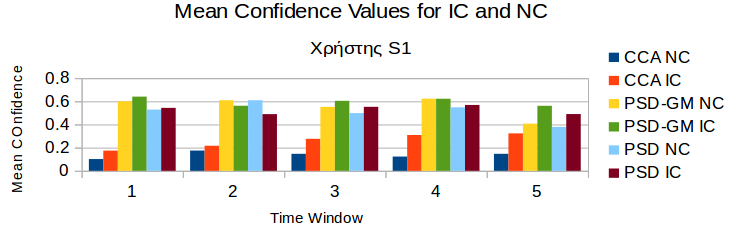
\includegraphics[scale=0.5]{{{ImagesSSVEP/S1_NC_THR}.png}}}
    \subfigure[]{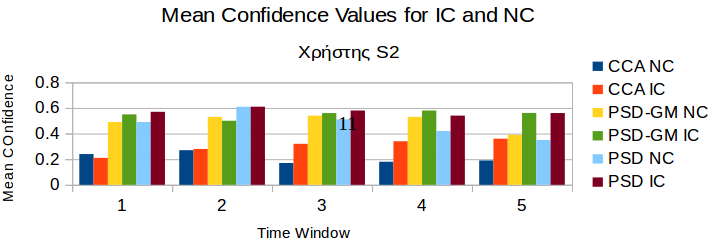
\includegraphics[scale=0.5]{{{ImagesSSVEP/S2_NC_THR}.png}}}
    \caption{Οι μέσες τιμές $confidence$ των εντολών NC και IC για κάθε μέθοδο και κάθε χρήστη.}
    \label{fig:thr_nc}
\end{figure}

\par Στα διαγράμματα των εικόνων \ref{fig:S1_NC} και \ref{fig:S2_NC}, φαίνονται τα αποτελέσματα ταξινόμησης για τους δύο χρήστες, όπου έχει συμπεριληφθεί και η αναγνώριση της εντολής NC. Παρατηρούμε αισθητή μείωση της συνολικής πιστότητας του συστήματος. Όπως αναμενόταν, οι PSD και PSD-GM μέθοδοι, δεν απέδωσαν καλά, και για τούς δύο χρήστες, σε αντίθεση με τον CCA, όπου για t=4sec, επιτεύχθηκε πιστότητα 75\% με ITR 12.01 bits/min για τον S1, και για t=5sec, 76\% με ITR 9.89 bits/min για τον S2. Τέλος, η συνδυαστική μέθοδος PSD-PCA-MLR-kNN, ήταν η μόνη που δεν βασιζόταν στον δείκτη confidence, και δεν είχε την αντίστοιχη επιτυχία που είχε στην ταξινόμηση των IC σημάτων στην προηγούμενη παράγραφο. Όπως έχουμε αναφέρει και προηγουμένως, το ελάχιστο αποδεκτό ποσοστό πιστότητας για μια BCI διεπαφή είναι το 70\%, συνεπώς η μέθοδος που θα δοκιμαστεί για το online σκέλος της διεπαφής, θα είναι η CCA.
\begin{figure}[H]
    \centering     %%% not \center
     \textbf{Χρήστης S1 (IC + NC)}\par\medskip
    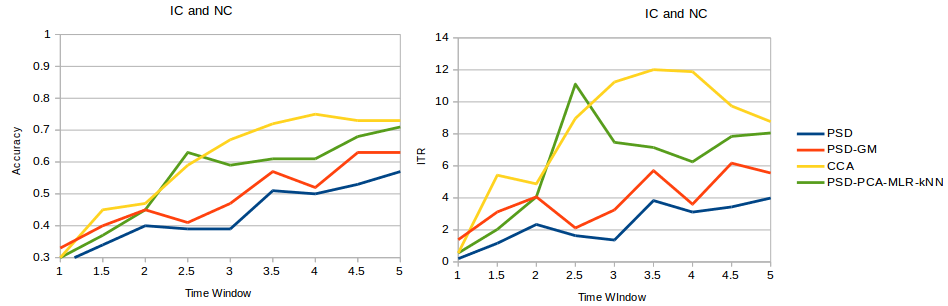
\includegraphics[scale=0.5]{{{ImagesSSVEP/S1_NC}.png}}
    \caption{Οι καμπύλες πιστότητας και ITR, του χρήστη S1 , για διαφορετικές τιμές χρονικού παραθύρου, όπου έχει συμπεριληφθεί και η αναγνώριση της εντολής NC.}
    \label{fig:S1_NC}
\end{figure}

\begin{figure}[H]
    \centering     %%% not \center
     \textbf{Χρήστης S2 (IC + NC)}\par\medskip
    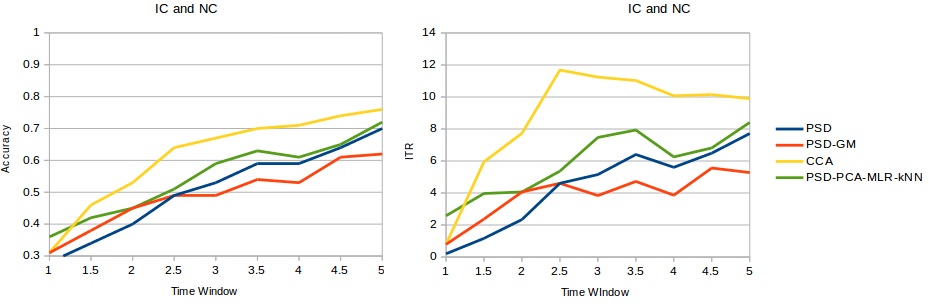
\includegraphics[scale=0.5]{{{ImagesSSVEP/S2_NC}.png}}
    \caption{Οι καμπύλες πιστότητας και ITR, του χρήστη S2, για διαφορετικές τιμές χρονικού παραθύρου, όπου έχει συμπεριληφθεί και η αναγνώριση της εντολής NC.}
    \label{fig:S2_NC}
\end{figure}

\par Τέλος, σχετικά με την NC εντολή, αξίζει να αναφερθούμε και στον ρυθμό των false positives (FPR). Η αλήθεια είναι πως τα ποσοστά ταξινόμησης που παρουσιάστηκαν προηγουμένως δεν αντιπροσωπεύουν την πλήρη εικόνα των αποτελεσμάτων. Ανάλογα με την κρισιμότητά της διεργασίας που επιτελείται μέσω της online διεπαφή, ο χρήστης έχει δύο βασικές απαιτήσεις, α) πολύ μικρό FPR, δηλαδή το σύστημα να μην παράγει κάποια έξοδο όταν ο χρήστης δεν το χρησιμοποιεί και β) Το σύστημα να ανιχνεύει με ψηλό ποσοστό επιτυχίας τις υπόλοιπες εντολές (SSVEP), δηλαδή χαμηλό  missclasification rate για τις IC εντολές. Ιδανικά, αν για μια εντολή, πρόκειται να συμβεί κάποιο missclasification, θα θέλαμε αυτή να ανιχνευτεί ως NC, έτσι ώστε το σύστημα απλά να μείνει αδρανές. Προκειμένου να ελέγξουμε κατά πόσο ικανοποιούνται αυτές οι απαιτήσεις, από την μέθοδο που απέδωσε καλύτερα στην ταξινόμηση των IC και NC εντολών για τον χρήστη S1 (CCA), παραθέτουμε τον Πίνακα Σύγχυσης (Confusion Matrix) \ref{tab:confusion}, για χρονικό παράθυρο t=4sec. 

\begin{table}[H]
    \centering
    \begin{tabular}{|c||*{5}{c|}}\hline
    \diagbox[]{Decision}{Intention}
    &\makebox[3em]{$f_1$}&\makebox[3em]{$f_2$}&\makebox[3em]{$f_3$}
    &\makebox[3em]{$f_4$}&\makebox[3em]{NC}\\\hline\hline
    $f_1$& 14& 0& 0& 0&  0\\\hline
    $f_2$&  0& 15& 0& 0& 0\\\hline
    $f_3$&  0& 0& 15& 0& 0\\\hline
    $f_4$&  0& 0& 0& 12& 1\\\hline
    NC&     6& 5& 5& 8& 19\\\hline
    \end{tabular}

    \caption{Πίνακας Σύγχυσης (Confusion Matrix) της ταξινόμησης IC και NC σημάτων, για τον χρήστη S1 για χρονικό παράθυρο t=4sec.}
    \label{tab:confusion}
\end{table}

\par Όπως φαίνεται, παρά σχετικά χαμηλό συνολικό accuracy (75\%), έχουμε false positive rate 5\% και missclasification rate 0\%, μεταξύ των IC εντολών ($f_1,f_2,f_3,f_4$), συνεπώς ο CCA είναι κατάλληλος για την υλοποίηση μια αξιόπιστης online BCI εφαρμογής. Τέλος να αναφέρουμε πως θα μπορούσαμε να εξαλείψουμε εντελώς τα false positives, αν αυξάναμε το κατώφλι $NC_{thr}$, ωστόσο, θα μειωνόταν σημαντικά η συνολική πιστότητα, και το σύστημα θα γινόταν αρκετά αργό και δύσκολο στην χρήση.

\subsection{Αποτελέσματα για κύματα Άλφα, t=1-5sec}
\par Το τελευταίο στάδιο πριν περάσουμε στην αξιολόγηση της online διεπαφής, είναι να υλοποιήσουμε και την μέθοδο ανίχνευσης άλφα κυμάτων, επιτρέποντας να προσθέσουμε μια ακόμα εντολή στην διεπαφή. Όπως αναφέραμε και στην ενότητα \ref{sec:online_design}, θα θεωρούμε πως ο χρήστης παράγει άλφα κύματα (κλειστά μάτια), όταν η μέση ενέργειά τους, υπερβαίνει ένα προκαθορισμένο κατώφλι $Alpha_{thr}$. Προς αυτή την κατεύθυνση, στην εικόνα \ref{fig:alpha_thr}, παρουσιάζουμε και για τους δύο χρήστες, την μέση τιμή της ενέργειας στην ζώνη συχνοτήτων 10-12Hz, για ανοιχτά και κλειστά μάτια. 

\begin{figure}[H]
    \centering     %%% not \center
    %\textbf{Χρήστης S2 (IC + NC)}\par\medskip
    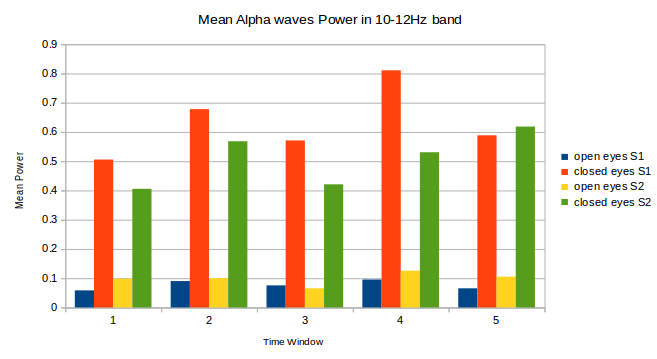
\includegraphics[scale=0.5]{{{ImagesSSVEP/alpha_thr}.png}}
    %\subfigure[]{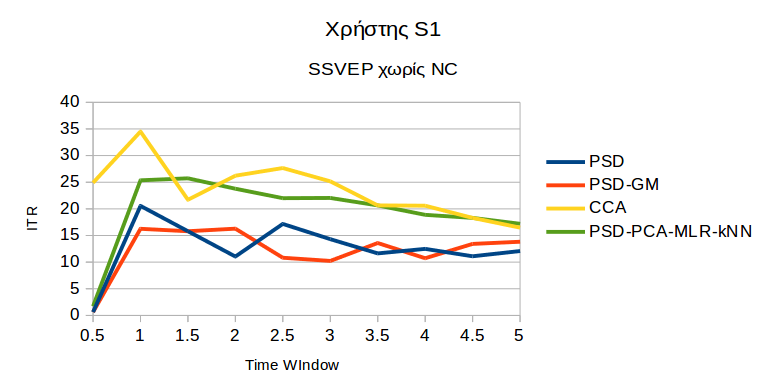
\includegraphics[scale=0.5]{{{ImagesSSVEP/S1_ITR}.png}}}
    \caption{Μέση τιμή της ενέργειας στην ζώνη 10-12Hz, των epoch που αντιστοιχούν σε ανοιχτά και κλειστά μάτια, για κάθε χρήστη και για διαφορετικά χρονικά παράθυρα.}
    \label{fig:alpha_thr}
\end{figure}

\par Όπως είναι αντιληπτό, η μέση ενέργεια στην ζώνη 10-12Hz αποτελεί ένα πολύ καλό κριτήριο διαχωρισμού των δύο αυτών καταστάσεων, και επιλέγοντας κατώφλι $Alpha_{thr}=0.25$, πετύχαμε ποσοστό επιτυχίας $98.125\%$ και $96.875\%$ για τους S1 και S2, αντίστοιχα. Εδώ να αναφέρουμε, σύμφωνα με το πρωτόκολλο καταγραφής, σε κάθε συνεδρία έχουμε 120 epochs, από τα οποία μόνο τα 20 αντιστοιχούν σε κλειστά μάτια, ενώ τα υπόλοιπα 100 σε ανοιχτά. Προκειμένου να κάνουμε ισοστάθμιση των δύο συνόλων, συμπεριλάβαμε epochs κλειστών ματιών, και από τις υπόλοιπες 3 συνεδρίες που είχαμε αρχικά απορρίψει για τον καθέναν. Συνεπώς τελικά είχαμε 80 epochs για κλειστά μάτια, και από την επιλεγμένη συνεδρία κάθε χρήστη, κρατήσαμε και 80 για ανοιχτά.

\textbf{Παρατήρηση}
\par Μετά και την προσθήκη της εντολής των κλειστών ματιών, πλέον έχουμε 5 Intentional Control (IC) εντολές (αντί για 4), και καθώς το ποσοστό αναγνώρισης των alpha κυμάτων είναι σχεδόν 100\%, επηρεάζει προς τα πάνω και την συνολική πιστότητα του συστήματος. Συνεπώς στην πράξη, ο ITR του οnline συστήματος, θα είναι υψηλότερος, σε σχέση με την περίπτωση των τεσσάρων IC.

\section{Αξιολόγηση Online διεπαφής}

\par Έπειτα από την offline ανάλυση, είναι ξεκάθαρο πως η απόδοση του CCA, αν και δεν ήταν η καλύτερη σε όλες τις περιπτώσεις, παρουσίασε την μεγαλύτερη σταθερότητα, και επίσης ήταν η μόνη μέθοδος που αναγνώριζε την NC εντολή με αποδεκτή αξιοπιστία. Η συνδυαστική μέθοδος PSD-PCA-MLR-kNN, έδωσε πολύ παρόμοια αποτελέσματα στην ταξινόμηση των IC σημάτων, χωρίς την αντίστοιχη επιτυχία όμως όταν λάβαμε υπόψιν μας και την NC. Επιπλέον, η συνδυαστική μέθοδος είναι πολύ πιο υπολογιστικά ακριβή από την CCA, καθώς και λιγότερο ευέλικτη, αφού χρειάζεται πρώτα ένα στάδιο εκπαίδευσης. Λαμβάνοντας υπόψιν μας τα παραπάνω, καθώς και το γεγονός πως δεν επιτυγχάνει καλύτερα αποτελέσματα από την CCA, μας οδήγησε στην μη χρήση της στο online σκέλος της διεπαφής.

\par Όπως αναφέρθηκε και στο κεφάλαιο \ref{chap:Background}, η χρήση της μετρικής ITR δεν αποτελεί έγκυρο τρόπο αξιολόγησης ενός ασύγχρονου (ή ενός constantly engaged) συστήματος πραγματικού χρόνου όπως αυτό που υλοποιήσαμε. Συνεπώς, σύμφωνα με την δημοσίευση, \cite{Yuan2013-jp}, ως μέτρο επίδοσης της διεπαφής μας, ορίσαμε τον χρόνο που απαιτείται για την ολοκλήρωση μιας συγκεκριμένης διαδικασίας από τον χρήστη, όπως η εύρεση του σωστού μονοπατιού σε έναν λαβύρινθο.

\par Στον πίνακα που ακολουθεί, παρουσιάζονται οι επιδόσεις κάθε χρήστη, για δύο εκδοχές του συστήματος, μια ασύγχρονη που περιλάμβανε την εντολή NC, και μία constantly engaged, χωρίς την δυνατότητα χρήστης της NC. Επιπλέον, καταγράψαμε το πλήθος των φορών που χρειάστηκε να γίνει αναίρεση κάποιας εντολής, καθώς και μια βαθμολογία που έδωσε ο κάθε χρήστης στο σύστημα, σχετικά με την ευκολία της χρήσης του (άριστα το 5).
\begin{table}[H]
    \centering
    \begin{tabular}{ |p{1cm}||p{1cm}|p{1cm}|p{1cm}|p{1cm}|p{1cm}|p{1cm}|}
        \hline
        & \multicolumn{3}{c|}{Asynchronous} & \multicolumn{3}{c|}{constantly engaged} \\
        \hline
        & \multicolumn{1}{c|}{Time (sec)} & \multicolumn{1}{c|}{Undo Commands} & \multicolumn{1}{c|}{Rating} & \multicolumn{1}{c|}{Time (sec)} & \multicolumn{1}{c|}{Undo Commands} &
        \multicolumn{1}{c|}{Rating} \\
        \hline
        S1          & 143& 0& 5& 74& 1& 4 \\
        S2          & 161& 2& 4& 104& 4& 2 \\
        \hline
        mean        & 152& 1& 4.5& 89& 2.5& 3\\
        \hline
    \end{tabular}
    \caption{Συγκεντρωτικά αποτελέσματα των χρόνων περάτωσης της πλοήγησης μέσα στον εικονικό λαβύρινθο, των εντολών αναίρεσης (κλειστά μάτια), καθώς και της βαθμολόγησης του συστήματος (άριστα το 5)}
    \label{tab:online}
\end{table}
\par Οι παράμετροι του συστήματος που χρησιμοποιήθηκαν για κάθε χρήστη, είναι:
\begin{itemize}
    \item \textbf{Χρήστης S1}
    \begin{itemize}
        \item Χρονικό παράθυρο : $t_w=4sec$
        \item Υπολογισμός κάθε : $t_r=0.5sec$
        \item Επικάλυψη μεταξύ παραθύρων : $ov = (t_w-t_r)/t_w=75\%$
        \item Μέγεθος buffer εντολών (\ref{fig:online_umls}b) : $k=3$
    \end{itemize}
    \item \textbf{Χρήστης S2}
    \begin{itemize}
        \item Χρονικό παράθυρο : $t_w=4sec$
        \item Υπολογισμός κάθε : $t_r=0.5sec$
        \item Επικάλυψη μεταξύ παραθύρων : $ov = (t_w-t_r)/t_w=90\%$
        \item Μέγεθος buffer εντολών (\ref{fig:online_umls}b) : $k=4$
    \end{itemize}
\end{itemize}

\par Σε μια προσπάθεια αξιολόγησης των παραπάνω χρόνων, θα προσπαθήσουμε να υπολογίσουμε τον ελάχιστο χρόνο ολοκλήρωσης της διαδικασίας κάτω από ιδανικές συνθήκες. Αυτός ο υπολογισμός είναι δυνατός μόνο για την περίπτωση του constantly engaged συστήματος, καθώς στο ασύγχρονο, η ύπαρξη της εντολής NC καθιστά τον υπολογισμό πολύ δύσκολο. Αρχικά υπολογίσαμε πως χρειάζονται 35 κινήσεις για να πάει το pacman στον στόχο. Για τον χρήστη S1, θεωρώντας πως έχουμε 100\% πιστότητα ταξινόμησης, τότε χρειάζονται $k\cdot t_r$ δευτερόλεπτα για κάθε μια εντολή, συνεπώς περίπου 52.5 δευτερόλεπτα συνολικά, ενώ αντίστοιχα για τον χρήστη S2, 70 δευτερόλεπτα. Δεδομένου τώρα πως το ποσοστό της offline ταξινόμησης για $t_w=4sec$, δεν ήταν 100\% αλλά 90\% (μόνο για τις IC), και ότι επίδοση των χρηστών κατά τις δοκιμές του online συστήματος μπορεί να είναι σημαντικά μικρότερη από αυτήν των offline δοκιμών, \cite{Muller-Putz2006-wj} \cite{Yuan2013-jp}, τα 86 και 92 δευτερόλεπτα που χρειάστηκαν οι χρήστης S1 και S2 αντίστοιχα, είναι αρκετά καλοί χρόνοι. 
%και υπάρχουν αρκετοί λόγοι γι' αυτό, όπως η διάσπαση της προσοχής του χρήστη λόγω της ανάδρασης του συστήματος (οθόνη, ενδείξεις κ.α)

\section{Γενικό Συμπέρασμα}

\par Τα παραπάνω προκαταρκτικά αποτελέσματα που παρουσιάστηκαν, καθιστούν σαφές πως ο Epoc μπορεί να χρησιμοποιηθεί για την ανίχνευση SSVEP σημάτων, καθώς και για την υλοποίηση απλών online διεπαφών.
\par Μια παρατήρηση είναι πως σε αντίθεση με τον χρήστη S2, o χρήστης S1 είχε περισσότερη εμπειρία στην χρήση διεπαφών SSVEP. Ίσως αυτός είναι και ο λόγος που ο S1 πέτυχε τα καλύτερα αποτελέσματα, σχεδόν σε όλες τις περιπτώσεις. Παρά το ότι γενικά δεν απαιτείται εκπαίδευση για την παραγωγή των SSVEPs, είναι γεγονός, πως ένας πιο έμπειρος χρήστης μπορεί να διαχειριστεί καλύτερα την κούραση που ίσως προκύψει κοιτώντας τις ΕΟΔ, καθώς επίσης έχει καλύτερο έλεγχο και συγκέντρωση κατά την διάρκεια της καταγραφής. Αυτό ίσως μπορεί να φανεί από τα αποτελέσματα του χρήστη S2 για τις συχνότητες $F_{mid}$ \ref{tab:full_results}. Για d.c 75\% τα αποτελέσματα είναι σημαντικά χαμηλότερα σε σχέση με αυτά που αντιστοιχούν σε d.c 50\%. Αυτή η διαφορά δεν μπορεί να αποδοθεί μόνο στο duty cycle, καθώς στην βιβλιογραφία δεν έχει αναφερθεί σε καμιά περίπτωση πως επηρεάζει τόσο σημαντικά τις επιδόσεις του συστήματος. Συνεπώς είναι πιθανόν ο χρήστης S2 να κουράστηκε και να μην ήταν συγκεντρωμένος κατά την διάρκεια της καταγραφής.

\par Τέλος, όπως έχουμε αναφέρει, η σύγκριση μεταξύ δύο BCI διεπαφών, είναι δύσκολη,  οι επιδόσεις του συστήματος μας συναγωνίζονται αυτές των δημοσιεύσεων \cite{Lin2014-cp}\cite{Liu2012-qj} που περιγράψαμε στο κεφάλαιο \ref{chap:survey}. Αν και στην  \cite{Liu2012-qj} αναφέρουν κατά μέσο όρο υψηλότερες ITR επιδόσεις, αυτό συμβαίνει επειδή διαχειρίζονται 6 IC εντολές, σε αντίθεση με τις 4 της εργασίας μας. Επιπλέον σε καμία από αυτές της εργασίες δεν έγινε δρομολόγηση του ζητήματος ανίχνευσης της NC κατάστασης, πρόβλημα το οποίο προσεγγίσαμε με σχετική επιτυχία για την CCA μέθοδο.

%Η μέθοδος PCA-MLR-kNN για την εξαγωγή χαρακτηριστικών από τα χρονικά σήματα, που προτάθηκε στη δημοσίευση \cite{Wang2016-nc} έδινε αποτελέσματα λίγο πάνω από το όριο τύχης (25\%) και δεν παρουσιάστηκε καθόλου. Αντιθέτως, όταν εφαρμόσαμε την ίδια τεχνική στα μετασχηματισμένα σήματα στην συχνότητα (PSD), τότε στην offline ανάλυση των IC σημάτων, ο χρήστης S1, πέτυχε την υψηλότερη πιστότητα, 91.25\% και ITR  17.19 bits/min,για t=5sec.

\end{document}